\documentclass{article}

\usepackage[version=3]{mhchem} % Package for chemical equation typesetting
\usepackage{siunitx} % Provides the \SI{}{} and \si{} command for typesetting SI units
\usepackage{natbib} % Required to change bibliography style to APA
\usepackage{graphicx}
\usepackage{mathtools}
\usepackage{amssymb}
\usepackage{amsthm}
\usepackage[italian]{babel}
\usepackage{stackengine}
\usepackage{graphicx,ifthen}
\usepackage{amsmath}
\usepackage{hyperref}
\usepackage{upgreek}
\usepackage{bm}

\renewcommand{\labelenumi}{\alph{enumi}.} % Make numbering in the enumerate environment by letter rather than number (e.g. section 6)

\title{Esperienza II: \\ interferometro}
\author{Manuel G. Moretti\footnote{email: manuel.moretti560@edu.unito.it}}
\date{Luglio 2024}

\begin{document}

\maketitle

\begin{center}
\begin{tabular}{l r}
Esperimentazioni II corso B & A.A. 2023/24 \\
Modulo II & Universit\'{a} degli Studi di Torino \\
\end{tabular}
\end{center}

\begin{abstract}
In questa esperienza si è stimata la lunghezza d'onda di un laser He-Ne attraverso l'utilizzo di un interferometro, osservando lo spostamento delle frange luminose del raggio sullo schermo. Sempre con lo stesso metodo e strumento si è determinato l'indice di rifrazione di una sottile lastra di vetro. Collegando infine una pompa a vuoto all'interferometro è stato possibile stimare l'indice di rifrazione dell'aria in funzione della pressione generata da essa. 
\end{abstract}

\section{Obiettivi della misura}
Gli obiettivi di questa esperienza sono di stimare la  lunghezza d'onda, misurare l'indice di rifrazione di una lastra di vetro e stimare l'indice di rifrazione dell'aria sfruttando un interferometro. 
\section{Configurazione dell'apparato sperimentale}
L'apparato sperimentale consiste in un laser He-Ne di lunghezza d'onda di $\lambda=(633\pm 1)$ nm e di un interferometro. Quest'ultimo è uno strumento dotato di una guida per il laser, di uno slot per inserire una sottile lente di vetro, di due specchi mobili, e di una lastra la cui funzione è di dividere il raggio in modo che esso colpisca i due specchi. Il raggio laser quindi si divide in due raggi ortogonali tra loro i quali colpiscono i due specchi. I due raggi quindi vengono riflessi da questi ultimi e ritornano sulla lastra separatrice, unendosi nuovamente in un unico raggio. Quest'ultimo raggio, generato dall'interferenza dei due precedenti, viene visualizzato su uno schermo, creando appunto una figura di interferenza ad anelli di Newton.

\section{Raccolta ed elaborazione dei dati}

\subsection{Stima della lunghezza d'onda del laser}
La raccolta dati per questa parte di esperienza è consistita in una serie conteggi del numero di frange $n_F$ che "scomparivano" al variare della posizione dello specchio perpendicolare al raggio laser (il secondo specchio è lasciato fisso). La variazione di posizione $\Delta x = x_0-x_f$ è misurata tramite un palmer con una precisione di un micron a partire dalla posizione iniziale $x_0$ di $(350\pm 1)\,\upmu\text{m}$. I risultati ottenuti sono raccolti nella seguente tabella.
\begin{table}[h]
    \centering
    \begin{tabular}{|c|c|c|c|}
        \hline
        \bm{$n_F$} & \bm{$x_0$} \textbf{[$\upmu$m]} & \bm{$x_f$} \textbf{[$\upmu$m]} & \bm{$\Delta x$} \textbf{[$\upmu$m]} \\
        \hline
        $70\pm 1$ & $350\pm 1$ & $328\pm 1$ & $22\pm 1$ \\
        \hline
        $75\pm 1$ & $350\pm 1$ & $326\pm 1$ & $24\pm 1$ \\
        \hline
        $80\pm 1$ & $350\pm 1$ & $325\pm 1$ & $25\pm 1$ \\
        \hline
    \end{tabular}
    \caption{Conteggio frange e variazione posizione specchio mobile}
    \label{tab:variazione posizione}
\end{table}

Quindi, muovendo lentamente lo specchio perpendicolare al raggio, la lunghezza d'onda del laser può essere stimata usando la relazione
\begin{equation}
    \label{eq:lambda laser}
    \lambda=\frac{2\Delta x}{n}.
\end{equation}

\subsection{Misura dell'indice di rifrazione di una lastra di vetro}
La raccolta dati per questa parte di esperienza è nuovamente consistita in una serie conteggi del numero di frange $n_F$ che "scomparivano" al variare dell'angolazione del parallelepipedo di vetro. La variazione di angolo $\Delta\theta$ è misurata tramite una scala graduata con una precisione di 0.1°. Inoltre, lo spessore della lastra di vetro è $d=(5.67\pm0.01)$ mm. I risultati ottenuti sono raccolti nella seguente tabella.
\begin{table}[h]
    \centering
    \begin{tabular}{|c|c|}
        \hline
        \bm{$n_F$} & \bm{$\Delta\theta$} \textbf{[deg]} \\
        \hline
        $55\pm1$ & $7.5\pm0.1$ \\
        \hline
        $55\pm1$ & $7.8\pm0.1$ \\
        \hline
        $55\pm1$ & $7.6\pm0.1$ \\
        \hline
    \end{tabular}
    \caption{Conteggio frange e variazione angolazione lastra}
    \label{tab:variazione angolazione}
\end{table}

Quindi, l'indice di rifrazione della lastra $n_l$ può essere stimata usando la relazione 
\begin{equation}
    \label{eq:n lastra}
    n_{sl}=\frac{\left(d-\frac{\lambda n_F}{2}\right)\left(1-\cos{\Delta\theta}\right)}{d\left(1-\cos{\Delta\theta}\right)-\frac{\lambda n_F}{2}},
\end{equation}

\subsection{Stima dell'indice di rifrazione dell'aria}
La raccolta dati per questa parte di esperienza è consistita in una serie conteggi del numero di frange $n_F$ che "scomparivano" al variare della pressione all'interno della camera a vuoto. La variazione di pressione $\Delta p$ è misurata, con una precisione di 0.1 bar, tramite una scala graduata di una valvola collegata al grilletto per creare il vuoto all'interno della camera. I risultati ottenuti sono raccolti nella seguente tabella\footnote{I valori di $n_F$ corrispondenti a valori negativi di pressione sono convenzionalmente posti anch'essi negativi in modo da poter ottenere una retta nel grafico in figura \ref{fig:grafico n(p)}}.
\begin{table}[h]
    \centering
    \begin{tabular}{|c|c|c|c|}
        \hline
        \bm{$n_F$} & \bm{$\Delta p$} \textbf{[bar]} \\
        \hline
        $-10\pm 1$ & $-0.6\pm 0.1$ \\
        \hline
        $47\pm 1$ & $2.5\pm 0.1$ \\
        \hline
        $37\pm 1$ & $2.0\pm 0.1$ \\
        \hline
        $40\pm 1$ & $2.1\pm 0.1$ \\
        \hline
        $-13\pm 1$ & $-0.8\pm 0.1$ \\
        \hline
    \end{tabular}
    \caption{Conteggio frange e variazione pressione}
    \label{tab:variazione pressione}
\end{table}

I dati raccolti nella tabella \ref{tab:variazione pressione} possono essere rappresentati in un grafico di $n_F$ in funzione della variazione di pressione $\Delta p$.
\begin{figure}[ht]
    \centering
    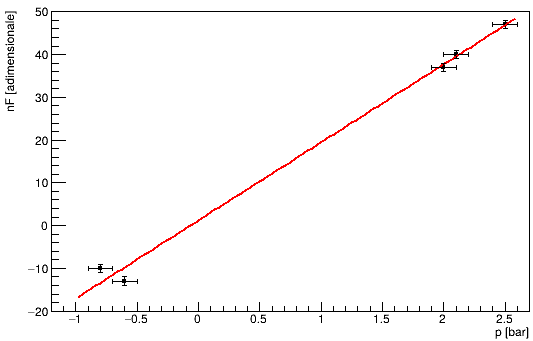
\includegraphics[width=0.7\linewidth]{Immagini/fit lineare int..png}
    \caption{grafico di $n_F(\Delta p)$}
    \label{fig:grafico n(p)}
\end{figure}

Quindi, dai dati raccolti nella tabella \ref{tab:variazione pressione} e dal coefficiente angolare $m$ della retta ricavata dal fit del grafico \ref{fig:grafico n(p)}, e usando la relazione
\begin{equation}
    \label{eq:n aria}
    n_{air}=n_{void}+\frac{\Delta n_F}{\Delta p}\frac{\lambda}{2s}=n_{void}+\frac{m\lambda}{2s},
\end{equation}
dove $s$ cm è lo spessore della camera a vuoto, è possibile ottenere una stima $n_{sa}$ dell'indice di rifrazione dell'aria $n_{air}$.

\section{Risultati e conclusioni}
Dai valori raccolti nella tabella \ref{tab:variazione posizione} e usando l'equazione \eqref{eq:lambda laser} si possono ottenere tre stime della lunghezza d'onda del laser
\begin{equation}
    \begin{cases}
        \lambda_1=(628\pm30) \,\text{nm} \\
        \lambda_2=(640\pm28) \,\text{nm} \\
        \lambda_3=(625\pm26) \,\text{nm}
    \end{cases}
\end{equation}
Effettuando dei test di Gauss tra le misure si trova che queste sono compatibili tra di loro, quindi è possibile mediarle ottenendo una stima $\lambda_s$ della lunghezza d'onda $\lambda$ del laser, in particolare
\begin{equation}
    \lambda_s=\frac{\lambda_1+\lambda_2+\lambda_3}{3}=(631\pm28)\,\unit{nm}.
\end{equation}
Questo valore può essere confrontato con il valore dichiarato dal costruttore di $\lambda=(633\pm1)$ nm svolgendo un test di Gauss. Il test restituisce un valore di $Z=0.07$, minore del valore critico $Z_c=1.96$ ad un livello di significatività del 5\%. In altre parole, questo significa che le due misure sono statisticamente compatibili.

Invece, dai valori raccolti nella tabella \ref{tab:variazione angolazione} e usando l'equazione \eqref{eq:n lastra} si possono ottenere tre stime dell'indice di rifrazione della lastra
\begin{equation}
    \begin{cases}
        n_1=(1.56\pm0.32) \\
        n_2=(1.49\pm0.37) \\
        n_3=(1.53\pm0.36)
    \end{cases}
\end{equation}
Effettuando dei test di Gauss tra le misure si trova che queste sono compatibili tra di loro, quindi è possibile mediarle ottenendo una stima $n_{ml}$ dell'indice di rifrazione $n_l$ della lastra di vetro
\begin{equation}
    n_{ml}=\frac{n_1+n_2+n_3}{3}=(1.53\pm0.20).
\end{equation}
Questo valore è in linea con i normali valori dell'indice di rifrazione del vetro che tende ad aggirarsi intorno ai valori di $n\approx1.6$.

Infine, sostituendo i valori di $m=(18.26\pm0.65)$, $s=(3.0\pm0.1)$ cm, $\lambda=(633\pm1)$ nm e $n_{void}=1$ nell'equazione \eqref{eq:stima n aria} si ottiene come stima dell'indice di rifrazione dell'aria il valore
\begin{equation}
    \label{eq:stima n aria}
    n_{sa}=(1.00019\pm0.00006).
\end{equation}
Effettuando un test Z tra la stima $n_{sa}$ e il valore noto di $n_{air}=(1.00029\pm0.00001)$ si trova un valore di $Z=1.64$, minore del valore critico $Z_c=1.96$ ad un livello di significatività del 5\%. In altre parole, questo significa che le due misure sono statisticamente compatibili.

\end{document}